\documentclass[11pt]{article}
\usepackage[margin=1.1in,headsep=18pt]{geometry}
\usepackage{amsmath, amsthm, amssymb}
\newcommand{\dgshorttitle}{The Floor Theorem at the Berger Field}
\newcommand{\dgauthorshort}{B. R. Davis}
% Davis Geometric house style, shared by the papers in docs/papers/.
% Loaded with % Davis Geometric house style, shared by the papers in docs/papers/.
% Loaded with % Davis Geometric house style, shared by the papers in docs/papers/.
% Loaded with \input{../dgstyle} after amsmath and amsthm (do not load amssymb: newpxmath provides it).
% Needs (TeX Live): newpx, titlesec, caption, fancyhdr, microtype, xcolor, enumitem.
\usepackage[T1]{fontenc}
\usepackage{newpxtext}
\usepackage[slantedGreek]{newpxmath}
\renewcommand{\ttdefault}{lmtt}  % Latin Modern typewriter for code and paths
\linespread{1.06}
\usepackage[final]{microtype}
\usepackage{xcolor}
\definecolor{dgink}{HTML}{1F2328}
\definecolor{dgmuted}{HTML}{5A5F66}
\definecolor{dgrule}{HTML}{C9CDD2}
\definecolor{dgchord}{HTML}{2A78D6}
\definecolor{dgarc}{HTML}{1BAF7A}
\definecolor{dgtan}{HTML}{EB6834}
\definecolor{dgblend}{HTML}{6250D6}
% headings: numbered small caps, quiet rules of space rather than ink
\usepackage{titlesec}
\titleformat{\section}{\normalfont\large\scshape\color{dgink}}{\thesection}{1em}{}
\titleformat{\subsection}{\normalfont\normalsize\itshape\color{dgink}}{\thesubsection}{0.8em}{}
\titleformat{\subsubsection}[runin]{\normalfont\normalsize\itshape}{\thesubsubsection}{0.6em}{}[.]
\titleformat{\paragraph}[runin]{\normalfont\normalsize\scshape}{}{0pt}{}  % sources end paragraph titles with their own stop
\titlespacing*{\section}{0pt}{2.4ex plus 0.6ex minus 0.3ex}{1.1ex plus 0.2ex}
\titlespacing*{\subsection}{0pt}{1.8ex plus 0.5ex minus 0.2ex}{0.7ex plus 0.2ex}
\titlespacing*{\paragraph}{0pt}{1.2ex plus 0.4ex minus 0.2ex}{0.6em}
% captions: small, label in small caps, ragged
\usepackage[font=small,labelfont=sc,labelsep=period,justification=justified,margin=4pt]{caption}
% running heads
\usepackage{fancyhdr}
\pagestyle{fancy}
\fancyhf{}
\renewcommand{\headrulewidth}{0pt}
\fancyhead[L]{\small\scshape\color{dgmuted}\dgauthorshort}
\fancyhead[R]{\small\itshape\color{dgmuted}\dgshorttitle}
\fancyfoot[C]{\small\color{dgmuted}\thepage}
\fancypagestyle{plain}{\fancyhf{}\fancyfoot[C]{\small\color{dgmuted}\thepage}}
\setlength{\headheight}{14pt}
% title block
\makeatletter
\renewcommand{\maketitle}{%
  \thispagestyle{plain}%
  \begin{center}
    {\LARGE\color{dgink}\@title\par}\vspace{1.1em}
    {\large\scshape\@author\par}\vspace{0.5em}
    {\small\color{dgmuted}\@date\par}
  \end{center}\vspace{0.6em}}
\renewenvironment{abstract}{%
  \begin{list}{}{\setlength{\leftmargin}{2.2em}\setlength{\rightmargin}{2.2em}}\item\relax
  \small\noindent{\scshape Abstract.}\enspace}{\end{list}\vspace{0.4em}}
\makeatother
\usepackage{enumitem}
\setlist{itemsep=0.25ex, topsep=0.6ex}
% "In plain words": a quiet ruled aside
\newenvironment{plain}{%
  \par\smallskip\begin{list}{}{\setlength{\leftmargin}{1.4em}\setlength{\rightmargin}{1.4em}}\item\relax
  \small\color{dgink}\noindent{\scshape In plain words.}\enspace}{\end{list}\smallskip}
 after amsmath and amsthm (do not load amssymb: newpxmath provides it).
% Needs (TeX Live): newpx, titlesec, caption, fancyhdr, microtype, xcolor, enumitem.
\usepackage[T1]{fontenc}
\usepackage{newpxtext}
\usepackage[slantedGreek]{newpxmath}
\renewcommand{\ttdefault}{lmtt}  % Latin Modern typewriter for code and paths
\linespread{1.06}
\usepackage[final]{microtype}
\usepackage{xcolor}
\definecolor{dgink}{HTML}{1F2328}
\definecolor{dgmuted}{HTML}{5A5F66}
\definecolor{dgrule}{HTML}{C9CDD2}
\definecolor{dgchord}{HTML}{2A78D6}
\definecolor{dgarc}{HTML}{1BAF7A}
\definecolor{dgtan}{HTML}{EB6834}
\definecolor{dgblend}{HTML}{6250D6}
% headings: numbered small caps, quiet rules of space rather than ink
\usepackage{titlesec}
\titleformat{\section}{\normalfont\large\scshape\color{dgink}}{\thesection}{1em}{}
\titleformat{\subsection}{\normalfont\normalsize\itshape\color{dgink}}{\thesubsection}{0.8em}{}
\titleformat{\subsubsection}[runin]{\normalfont\normalsize\itshape}{\thesubsubsection}{0.6em}{}[.]
\titleformat{\paragraph}[runin]{\normalfont\normalsize\scshape}{}{0pt}{}  % sources end paragraph titles with their own stop
\titlespacing*{\section}{0pt}{2.4ex plus 0.6ex minus 0.3ex}{1.1ex plus 0.2ex}
\titlespacing*{\subsection}{0pt}{1.8ex plus 0.5ex minus 0.2ex}{0.7ex plus 0.2ex}
\titlespacing*{\paragraph}{0pt}{1.2ex plus 0.4ex minus 0.2ex}{0.6em}
% captions: small, label in small caps, ragged
\usepackage[font=small,labelfont=sc,labelsep=period,justification=justified,margin=4pt]{caption}
% running heads
\usepackage{fancyhdr}
\pagestyle{fancy}
\fancyhf{}
\renewcommand{\headrulewidth}{0pt}
\fancyhead[L]{\small\scshape\color{dgmuted}\dgauthorshort}
\fancyhead[R]{\small\itshape\color{dgmuted}\dgshorttitle}
\fancyfoot[C]{\small\color{dgmuted}\thepage}
\fancypagestyle{plain}{\fancyhf{}\fancyfoot[C]{\small\color{dgmuted}\thepage}}
\setlength{\headheight}{14pt}
% title block
\makeatletter
\renewcommand{\maketitle}{%
  \thispagestyle{plain}%
  \begin{center}
    {\LARGE\color{dgink}\@title\par}\vspace{1.1em}
    {\large\scshape\@author\par}\vspace{0.5em}
    {\small\color{dgmuted}\@date\par}
  \end{center}\vspace{0.6em}}
\renewenvironment{abstract}{%
  \begin{list}{}{\setlength{\leftmargin}{2.2em}\setlength{\rightmargin}{2.2em}}\item\relax
  \small\noindent{\scshape Abstract.}\enspace}{\end{list}\vspace{0.4em}}
\makeatother
\usepackage{enumitem}
\setlist{itemsep=0.25ex, topsep=0.6ex}
% "In plain words": a quiet ruled aside
\newenvironment{plain}{%
  \par\smallskip\begin{list}{}{\setlength{\leftmargin}{1.4em}\setlength{\rightmargin}{1.4em}}\item\relax
  \small\color{dgink}\noindent{\scshape In plain words.}\enspace}{\end{list}\smallskip}
 after amsmath and amsthm (do not load amssymb: newpxmath provides it).
% Needs (TeX Live): newpx, titlesec, caption, fancyhdr, microtype, xcolor, enumitem.
\usepackage[T1]{fontenc}
\usepackage{newpxtext}
\usepackage[slantedGreek]{newpxmath}
\renewcommand{\ttdefault}{lmtt}  % Latin Modern typewriter for code and paths
\linespread{1.06}
\usepackage[final]{microtype}
\usepackage{xcolor}
\definecolor{dgink}{HTML}{1F2328}
\definecolor{dgmuted}{HTML}{5A5F66}
\definecolor{dgrule}{HTML}{C9CDD2}
\definecolor{dgchord}{HTML}{2A78D6}
\definecolor{dgarc}{HTML}{1BAF7A}
\definecolor{dgtan}{HTML}{EB6834}
\definecolor{dgblend}{HTML}{6250D6}
% headings: numbered small caps, quiet rules of space rather than ink
\usepackage{titlesec}
\titleformat{\section}{\normalfont\large\scshape\color{dgink}}{\thesection}{1em}{}
\titleformat{\subsection}{\normalfont\normalsize\itshape\color{dgink}}{\thesubsection}{0.8em}{}
\titleformat{\subsubsection}[runin]{\normalfont\normalsize\itshape}{\thesubsubsection}{0.6em}{}[.]
\titleformat{\paragraph}[runin]{\normalfont\normalsize\scshape}{}{0pt}{}  % sources end paragraph titles with their own stop
\titlespacing*{\section}{0pt}{2.4ex plus 0.6ex minus 0.3ex}{1.1ex plus 0.2ex}
\titlespacing*{\subsection}{0pt}{1.8ex plus 0.5ex minus 0.2ex}{0.7ex plus 0.2ex}
\titlespacing*{\paragraph}{0pt}{1.2ex plus 0.4ex minus 0.2ex}{0.6em}
% captions: small, label in small caps, ragged
\usepackage[font=small,labelfont=sc,labelsep=period,justification=justified,margin=4pt]{caption}
% running heads
\usepackage{fancyhdr}
\pagestyle{fancy}
\fancyhf{}
\renewcommand{\headrulewidth}{0pt}
\fancyhead[L]{\small\scshape\color{dgmuted}\dgauthorshort}
\fancyhead[R]{\small\itshape\color{dgmuted}\dgshorttitle}
\fancyfoot[C]{\small\color{dgmuted}\thepage}
\fancypagestyle{plain}{\fancyhf{}\fancyfoot[C]{\small\color{dgmuted}\thepage}}
\setlength{\headheight}{14pt}
% title block
\makeatletter
\renewcommand{\maketitle}{%
  \thispagestyle{plain}%
  \begin{center}
    {\LARGE\color{dgink}\@title\par}\vspace{1.1em}
    {\large\scshape\@author\par}\vspace{0.5em}
    {\small\color{dgmuted}\@date\par}
  \end{center}\vspace{0.6em}}
\renewenvironment{abstract}{%
  \begin{list}{}{\setlength{\leftmargin}{2.2em}\setlength{\rightmargin}{2.2em}}\item\relax
  \small\noindent{\scshape Abstract.}\enspace}{\end{list}\vspace{0.4em}}
\makeatother
\usepackage{enumitem}
\setlist{itemsep=0.25ex, topsep=0.6ex}
% "In plain words": a quiet ruled aside
\newenvironment{plain}{%
  \par\smallskip\begin{list}{}{\setlength{\leftmargin}{1.4em}\setlength{\rightmargin}{1.4em}}\item\relax
  \small\color{dgink}\noindent{\scshape In plain words.}\enspace}{\end{list}\smallskip}

\usepackage{graphicx}
\usepackage{booktabs}
\usepackage{url}
\usepackage[hidelinks]{hyperref}

\newtheorem{theorem}{Theorem}[section]
\newtheorem{proposition}[theorem]{Proposition}
\newtheorem{lemma}[theorem]{Lemma}
\newtheorem{corollary}[theorem]{Corollary}
\theoremstyle{definition}
\newtheorem{definition}[theorem]{Definition}
\theoremstyle{remark}
\newtheorem{remark}[theorem]{Remark}


% Redline of the review of 20 November 2026 (third round: Astra's adversarial review of version 2). \redlinetrue
% shows the changes (insertions blue, deletions red and struck out); \redlinefalse gives the accepted text.
\usepackage[normalem]{ulem}
\newif\ifredline
\redlinetrue
\newcommand{\redins}[1]{\ifredline{\color{blue}#1}\else#1\fi}
\newcommand{\reddel}[1]{\ifredline{\color{red}\sout{#1}}\fi}

\newcommand{\su}{\mathfrak{su}(2)}
\newcommand{\norm}[1]{\lVert #1\rVert}
\newcommand{\RR}{\mathbb{R}}

\title{The Floor Theorem for the Yang--Mills Hessian\\ at the Berger Field\\[4pt]
\large A Floor Law Across the Berger Spheres}
\author{Bee Rosa Davis\\[1pt] {\normalsize\upshape\itshape Davis Geometric}\\[1pt]
{\footnotesize\upshape ORCID \href{https://orcid.org/0009-0009-8034-4308}{0009-0009-8034-4308}}}
\date{November 2026 (version 2)}

\begin{document}
\maketitle

\begin{abstract}
Let $A$ be the Levi-Civita connection of the Berger metric $g=(3,1,1)$ on $S^3=SU(2)$, viewed as an
$SU(2)$ connection. It is not a Yang--Mills critical point. We compute the low spectrum of the Hessian
of the Yang--Mills energy at $A$, compressed to the gauge-orthogonal slice. The operator splits into
finite sectors by the Peter--Weyl decomposition. In the sector of spin $j/2$, the field
$f\,(\hat\theta^1+i\hat\theta^2)\otimes(\tau_1+i\tau_2)$, with $f$ the top weight along the long axis,
is an exact eigenvector with eigenvalue $(j(j+2)-14)/3$, orthogonal to every gauge direction. A
Weitzenb\"ock identity, proved in the universal enveloping algebra, bounds every sector from below.
Together with certified inertia counts in interval arithmetic, it shows that this value is the bottom of
its sector for the sectors $j=0,12,20,24$ that survive on the Poincar\'e homology sphere $S^3/2I$, and
that every other surviving sector lies above $142$. There, the
gauge-orthogonal spectrum below $142$ consists of the left-invariant values $-14/3$ (twice),
$16-2\sqrt{73}$, $22/3$ (twice) and $16+2\sqrt{73}$, and the spin-$6$ values from $154/3$ upward. The
first sector above the left-invariant one begins $168/3$ above the field's growth mode\redins{ (its lowest, negative eigenvalue)}, one third of
the sphere's first scalar eigenvalue. The construction reproduces the published fluctuation spectrum
of the meron on the round sphere and Laquer's index. The formula is one member of a family: on every
Berger sphere $(t,1,1)$ the same field is an exact gauge-orthogonal eigenvector with eigenvalue
$[j(j+2)-2(t-3)j-2(t-2)(t+4)]/t$. It is the floor of every sector
for every $t\in[2.75,10]$, in particular at $t=3$: a conserved charge splits each sector into blocks of size at most
nine, interval certificates of the blocks cover $j<100$, and a closed-form Gershgorin bound covers $j\ge100$.
 At $t=4$ the low spectrum on the
Poincar\'e sphere is classified below $136$. To our knowledge, these are the first exact eigenvalues of a
Yang--Mills Hessian at a non-flat connection on a squashed three-sphere.
\end{abstract}

\noindent\textbf{Keywords.} Yang--Mills Hessian; Berger sphere; Poincar\'e homology sphere; spectral
gap; Peter--Weyl decomposition; Weitzenb\"ock identity; computer-assisted proof.

\noindent\textbf{MSC 2020.} 58J50, 81T13, 58E15, 53C30, 65G30.

\section{Introduction}\label{sec:intro}

The second variation of the Yang--Mills energy decides whether a connection is a local minimum, how
fast nearby fields grow or decay under the gradient flow, and what spectral observables a lattice
discretization must reproduce. At Yang--Mills fields on round spheres and symmetric spaces it is
classical. Bourguignon and Lawson~\cite{bl1981} studied stability and isolation over the round
sphere and other locally homogeneous spaces. Laquer~\cite{laquer1984} computed the index and nullity
of the canonical connection over every simply connected compact irreducible symmetric space; for a
group manifold the index is one (see also~\cite{ohnitapan1989}). Around homogeneous backgrounds on
the round $S^3$, Kumar, Lechtenfeld and Pican\c{c}o Costa~\cite{klc2021} diagonalized the
fluctuation operator sector by sector in closed form. On Berger spheres, closed-form spectra are known
for the scalar Laplacian~\cite{lauret2019}, the Dirac operator~\cite{hitchin1974,bar1992,klingschueth2022} and
the Hodge Laplacian on $1$-forms~\cite{henkellauret2026}.

We found no exact result for the Yang--Mills Hessian at a non-flat connection on a squashed
three-sphere, nor at a connection that is not a Yang--Mills field. At the flat connection the Hessian
on coexact $\su$-valued $1$-forms is $d^*d$ tensored with $\su$, so its spectrum on a Berger sphere follows
from the Hodge spectrum of~\cite{henkellauret2026}. This paper supplies one, at the natural candidate: the Levi-Civita
connection of a Berger metric, viewed as an $SU(2)$ connection (the \emph{Berger field}). It arises as
the instantaneous state of a homogeneous gauge field transported along the Ricci flow of the
metric~\cite{davisrtc}, and it is the background on which lattice Yang--Mills forces on the
Poincar\'e homology sphere were tested there. Its exact spectrum gives those computations a target.

\paragraph{Main results.} Section~\ref{sec:setting} fixes the operator: the Hessian $H$ of the energy
at the Berger field, against the $L^2$ mass, compressed to the gauge-orthogonal slice. The field is not
at rest, so gauge directions are not zero modes, and the compression $PHP$ is the object studied.
\begin{itemize}
  \item \emph{The left-invariant sector} (Section~\ref{sec:spin0}) is computed exactly. Three of its
    nine directions are gauge directions. Its slice spectrum is $-14/3$ (twice), $16-2\sqrt{73}$,
    $22/3$ (twice) and $16+2\sqrt{73}$. All three growth directions come from the commutator.
  \item \emph{The floor formula} (Proposition~\ref{prop:bottom}): in every sector, $(j(j+2)-14)/3$ is an
    exact eigenvalue, on an explicit eigenvector orthogonal to the gauge directions. That it is the bottom of
    its sector is proved for $j=0,12,20,24$ (Theorem~\ref{thm:gap}), with a gap of $1/3$, and for every $j$ by
    Theorem~\ref{thm:range}.
  \item \emph{A Weitzenb\"ock identity} (Lemma~\ref{lem:weitz}), proved in $U(\su)$, gives a lower
    bound for every sector at once.
  \item \emph{The Floor Theorem} (Theorem~\ref{thm:gap}) follows, with certified
    inertia counts in the four sectors that matter.
  \item \emph{The floor law} (Section~\ref{sec:family}): the formula extends to every Berger sphere $(t,1,1)$
    as an exact eigenvalue (Proposition~\ref{prop:family}). It is certified as the floor at $t=4$
    (Theorem~\ref{thm:t4}) and for every $t\in[2.75,10]$ in every sector
    (Theorem~\ref{thm:range}); its eigenvector is a lowest Landau level, annihilated by the transverse
    raising operator, with its internal frame the lowest eigenvector of the curvature term of the Weitzenb\"ock
    identity\redins{ for $t\ge12/7$, so on the whole certified range}
    (Proposition~\ref{prop:landau}),
    with the stretches at which each twist \redins{(the circular field of Proposition~\ref{prop:bottom}; terms in Section~\ref{sec:setting}) }goes free in closed form (Corollary~\ref{cor:family}).
\end{itemize}
Section~\ref{sec:family} follows the floor across the Berger family.
Section~\ref{sec:checks} checks the construction against the published round-sphere results and
against lattice computations. Section~\ref{sec:discussion} states the scope.

\section{Setting}\label{sec:setting}

\paragraph{Frame and metric.} On $S^3=SU(2)$ let $e_0,e_1,e_2$ be a left-invariant frame with
$[e_a,e_b]=2\varepsilon_{abc}e_c$. The Berger metric is diagonal in it, with $g_0=3$ and $g_1=g_2=1$;
$\hat e_i=e_i/\sqrt{g_i}$ is orthonormal, with coframe $\hat\theta^i$ and structure constants
$[\hat e_i,\hat e_j]=\sum_kc_{ij}^{\,k}\hat e_k$, $c_{ij}^{\,k}=2\varepsilon_{ijk}\sqrt{g_k}/\sqrt{g_ig_j}$.

\paragraph{The Berger field.} The Levi-Civita connection has Christoffel symbols
$\Gamma_{ijk}=\tfrac12(c_{ij}^{\,k}-c_{jk}^{\,i}+c_{ki}^{\,j})$ in the orthonormal frame. Identifying
$\mathfrak{so}(3)$ with $\su$, write it as the $\su$-valued $1$-form $A=\sum_iM_i\hat\theta^i$ with
constant $M_i$, where $\tau_0,\tau_1,\tau_2$ is a basis of $\su$ with the same brackets as the frame,
$\tau_0$ along the long axis.
Its curvature $F$ has components $F_{ij}=[M_i,M_j]-\sum_kc_{ij}^{\,k}M_k$. At the round metric $A$ is
a Yang--Mills field; at $g=(3,1,1)$ it is not.

\redins{\paragraph{Terms.} A field is \emph{at rest} if it is a Yang--Mills field, a critical point of the
energy. A \emph{growth mode} is a direction of negative second variation, a negative eigenvalue of the Hessian
below. The \emph{stretch} is the parameter $t$ of the Berger metric $(t,1,1)$ of Section~\ref{sec:family}; the
main case is $t=3$. The \emph{twist} of the sector of spin $j/2$ is the field
$b=f\,(\hat\theta^1+i\hat\theta^2)\otimes(\tau_1+i\tau_2)$ of Proposition~\ref{prop:bottom}, with $f$ the top
weight along the long axis: it turns in the two short directions and, in step, in two internal directions. A
twist \emph{goes free} at the stretch where its eigenvalue crosses zero; beyond it, it is a growth mode.

}\paragraph{The Hessian and the slice.} A variation is $b=\sum_ib_i\hat\theta^i$. The second variation
of $E=\tfrac12\norm{F}^2$ is the quadratic form
\begin{equation}\label{eq:Q}
  Q(b)=\sum_{i<j}\norm{D_{ij}b}^2+2\langle F_{ij},[b_i,b_j]\rangle,\qquad
  D_{ij}b=\hat e_ib_j-\hat e_jb_i+[M_i,b_j]-[M_j,b_i]-\textstyle\sum_kc_{ij}^{\,k}b_k,
\end{equation}
and $H$ is its operator against the $L^2$ mass $\sum_i\norm{b_i}^2$. The gauge map is
$G\xi=(\hat e_i\xi+[M_i,\xi])_i$ with $L^2$ adjoint $G^*$. Because $A$ is not at rest, $H$ does not
preserve $\ker G^*$. The \emph{gauge-orthogonal spectrum} is the spectrum of $PHP$ on $\ker G^*$, with
$P$ the $L^2$ projection.

\paragraph{Sectors.} Everything is invariant under left translations, so by Peter--Weyl the operators
split into sectors indexed by $j\ge0$. In the sector of spin $j/2$, $b_i\in V_j\otimes\su$, where
$V_j$ is the spin-$j/2$ representation (dimension $j+1$) on which $e_i$ acts by an anti-Hermitian
$\rho_i$ with $[\rho_a,\rho_b]=2\varepsilon_{abc}\rho_c$. So $H$ is a finite Hermitian matrix of size
$9(j+1)$. Write $J_0=\tfrac i2\rho_0$, with weights $-\tfrac j2,\dots,\tfrac j2$.

\paragraph{The Poincar\'e sphere.} The binary icosahedral group $2I$ acts by left translations, and
the frame, the metric and $A$ descend to $S^3/2I$. The sector of spin $j/2$ survives with
multiplicity $\dim V_j^{2I}$, given by the Molien series $(1+t^{30})/((1-t^{12})(1-t^{20}))$ of
\reddel{Klein's invariants~\cite{klein1884}}\redins{the binary icosahedral group, whose invariants go back to Klein~\cite{klein1884}}: the surviving sectors are $j=0,12,20,24,30,32,\dots$. The first
nonzero eigenvalue of the scalar Laplacian on the unit Poincar\'e sphere is $j(j+2)=168$ at
$j=12$~\cite{lachiezerey2004}.

\section{The left-invariant sector}\label{sec:spin0}

At $j=0$ the Hessian is a $9\times9$ matrix with entries in $\mathbb{Q}(\sqrt3)$, computed in exact
arithmetic.

\begin{proposition}\label{prop:spin0}
At $j=0$:
\begin{enumerate}
  \item the spectrum of $H$ is $-14/3$ $(\times2)$, $(29-\sqrt{1345})/3$ $(\times2)$, $16-2\sqrt{73}$,
    $8$, $(29+\sqrt{1345})/3$ $(\times2)$, $16+2\sqrt{73}$;
  \item the gauge directions are $b_i=[M_i,\xi]$, $\xi\in\su$, a three-dimensional space. The
    compression of $H$ to it has eigenvalues $8$, $12$, $12$. The value $8$ is an eigenvalue of $H$ with a
    purely gauge eigenvector; the two $12$s are values of the compression only, since $H$ does not preserve
    this space;
  \item the gauge-orthogonal spectrum is $-14/3$ $(\times2)$, $16-2\sqrt{73}$, $22/3$ $(\times2)$,
    $16+2\sqrt{73}$.
\end{enumerate}
\end{proposition}
\begin{proof}
Exact symbolic computation of~\eqref{eq:Q} and of the compression to the orthogonal complement of the
gauge span (\path{scripts/ricci_su2_left_invariant_sector.py},
\path{scripts/ricci_su2_sector_minimality.py}).
\end{proof}

The eigenvalue $8$ is a pure gauge direction, and the pairs $(29\mp\sqrt{1345})/3$ are mixtures, $40\%$
and $60\%$ gauge. So the \reddel{field}\redins{left-invariant sector} has exactly three \emph{physical} growth directions, $-14/3$ (twice) and
$16-2\sqrt{73}$, each orthogonal to the gauge directions.\redins{ On $S^3$ other sectors add more: at $t=3$ the
sectors $j=1$ and $j=2$ have four each, among them their twists (Corollary~\ref{cor:family}). On the Poincar\'e
sphere those sectors do not survive, and the three are all.} All of them come from the field acting on
itself: with the commutator dropped, the same sector is $4/3$ $(\times6)$ and $12$ $(\times3)$, all
positive.

\section{The floor formula}\label{sec:bottom}

\begin{proposition}[The floor formula]\label{prop:bottom}
In the sector of spin $j/2$, let $f\in V_j$ be the top weight, $J_0f=\tfrac j2f$. The field
\[
  b=f\,(\hat\theta^1+i\,\hat\theta^2)\otimes(\tau_1+i\,\tau_2)
\]
is an eigenvector of $H$, orthogonal to every gauge direction, with eigenvalue
$\lambda(j)=(j(j+2)-14)/3$.
\end{proposition}
\begin{proof}
At the top weight, $\hat e_0f=-ijf/\sqrt3$, $J_+f=0$, $\rho_2f=i\rho_1f$ and $\norm{\rho_1f}^2=j$. So
every term of~\eqref{eq:Q} on fields supported at the top weight involves only $f$ and
$u=\rho_1f/\sqrt j$, with coefficients polynomial in $j$. On the squashed plane (frame and Lie indices
$1,2$, in the order $(1,1),(1,2),(2,1),(2,2)$) the Hessian is
\[
  \Bigl(\tfrac{j^2}{3}+j\Bigr)I+\frac13\begin{pmatrix}14&2ij&-ij&28\\-2ij&5&-19&-ij\\ ij&-19&5&2ij\\
  28&ij&-2ij&14\end{pmatrix},
\]
with eigenvalues $\tfrac13(j^2+2j-14)$, $\tfrac13(j^2+4j-14)$ and
$\tfrac13\bigl(j^2+3j+33\pm3\sqrt{j^2+9}\bigr)$. The first has eigenvector $(-1,-i,-i,1)$, which is $b$
up to a factor.\redins{ The other three are eigenvalues of this compression only, not of $H$.} Three facts complete the argument, each an identity in $j$:
\begin{itemize}
  \item the coupling of $b$ to the only other top-weight direction it could reach, the $\tau_0$
    component of $b_0$, vanishes;
  \item $D_{ij}b$ has no component along $u$, because the two circular factors cancel, so $H$ maps $b$
    into the top weight;
  \item $\langle G\xi,b\rangle=0$ for every $\xi$, at every weight.
\end{itemize}
All of these are verified symbolically in $j$ (\path{scripts/ricci_su2_sector_formula.py}).
\end{proof}

At $j=0$ the proposition gives the growth mode $-14/3$. The circular field is the left-invariant growth
mode lifted to the top weight of each higher sector, and the lift costs exactly $j(j+2)/3$.

\section{The Weitzenb\"ock bound and the gap}\label{sec:gap}

On the slice $G^*b=0$, so $\langle b,Hb\rangle=\langle b,(H+GG^*)b\rangle$: adding the gauge term changes
nothing there. The operator $H+GG^*$ has a useful form.

\begin{lemma}[Weitzenb\"ock identity]\label{lem:weitz}
In every sector,
\[
  H+GG^*=\sum_iX_i^*X_i+R_0,\qquad X_i=\rho_i/\sqrt{g_i}+\Omega_i,
\]
where $X_i$ is the covariant derivative ($\Omega_i$ is the action of the connection on the Lie index
together with $-\Gamma_i$ on the frame index) and $R_0$ is a constant real symmetric $9\times9$ matrix
with eigenvalues $-12$ $(\times2)$, $7\pm\sqrt{73}$, $2\pm2\sqrt{13}$ $(\times2)$ and $8$. Moreover
$\omega^2:=\sum_i\norm{\Omega_i}\redins{_2}^2=76/3$\redins{ (operator norms)}.
\end{lemma}
\begin{proof}
Treat the $\rho_i$ as generators of $U(\su)$ with $[\rho_a,\rho_b]=2\varepsilon_{abc}\rho_c$ and
$\rho_i^*=-\rho_i$. Both sides are $9\times9$ matrices over $U(\su)$ of filtration degree at most two.
Put every product in Poincar\'e--Birkhoff--Witt order. Every coefficient of degree one and two then
agrees, and the constant terms differ by $R_0$, in exact arithmetic with $\sqrt3$ symbolic. By the PBW
theorem the identity holds in $U(\su)$, hence in every representation $V_j$
(\path{scripts/ricci_su2_gap_certificates.py}).
\end{proof}

\begin{theorem}[The Floor Theorem]\label{thm:gap}
At the Berger metric $g=(3,1,1)$:
\begin{enumerate}
  \item every gauge-orthogonal eigenvalue in the sector of spin $j/2$ is at least
    $\bigl(\sqrt{j(j+2)/3}-\omega\bigr)^2-12$, $\omega=\sqrt{76/3}$, whenever $\sqrt{j(j+2)/3}\ge\omega$;
  \item for $j=0,12,20,24$, $\lambda(j)$ is the lowest gauge-orthogonal eigenvalue of its sector, and every
    other eigenvalue of $H+GG^*$ is at least $\lambda(j)+1/3-10^{-53}$;
  \item on the Poincar\'e sphere, the gauge-orthogonal spectrum below $142$ consists of the spin-$0$
    values of Proposition~\ref{prop:spin0}(3) and the spin-$6$ values from $154/3$ upward; spin $10$
    begins exactly at $142$.
\end{enumerate}
\end{theorem}
\begin{proof}
\emph{Part (1).} Since $g_0=3\ge g_1=g_2=1$ and $-\sum_i\rho_i^2=j(j+2)$ on $V_j$,
$\sum_i\norm{\rho_iv}^2/g_i\ge j(j+2)\norm v^2/3$. Each term satisfies
$\norm{X_iv}\ge\bigl|\norm{\rho_iv}/\sqrt{g_i}-\norm{\Omega_iv}\bigr|$. The reverse triangle inequality
in $\RR^3$ gives $\sum_i\norm{X_iv}^2\ge(\sqrt{j(j+2)/3}-\omega)^2\norm v^2$. With
Lemma~\ref{lem:weitz} and $\langle b,Hb\rangle=\langle b,(H+GG^*)b\rangle$ on the slice, this is (1).

\emph{Part (2).} Write $A=H+GG^*$. By Proposition~\ref{prop:bottom}, $\lambda(j)$ is an eigenvalue of $A$
of multiplicity at least two: the eigenvector $b$ at the top weight, and its image at the bottom weight
under the real structure of the integer-spin representation, which commutes with $A$ because every
coefficient is real. The rest is a rigorous count of the eigenvalues of $A$ below $\mu=\lambda(j)+1/3$
(\path{scripts/ricci_su2_gap_certificates.py}; every quantity below is recorded in its receipt).
\begin{enumerate}
  \item \emph{Enclosure.} $A-\mu$ is assembled in interval arithmetic, in mpmath's interval context
    (outward-rounded endpoints, $200$ bits~\cite{mpmath}), with $\sqrt3$ and every entry enclosed. It is
    realified, $\mathbb C^n\to\RR^{2n}$ by $z\mapsto(\operatorname{Re}z,\operatorname{Im}z)$, so every
    eigenvalue of $A$ appears twice. Let $M$ be the real symmetric matrix of the \redins{stored (rounded) }midpoints of its lower
    triangle. The exact realified matrix is symmetric and each interval encloses its entry, so the two
    differ in norm by at most $\rho$, computed from the radii\redins{. Each radius bounds the distance from the
    interval to its stored midpoint, and is computed, like $\rho$ itself, with outward rounding}.
  \item \emph{Factorization.} $M$ is factored without pivoting in $200$-bit arithmetic\reddel{,
    $LDL^\top=M+\Delta M$, with $|\Delta M|\le\gamma_N|L||D||L^\top|$, $\gamma_N=Nu/(1-Nu)$,
    $u=2^{-200}$: the componentwise bound for Gaussian elimination, applied
    to the symmetric elimination}\redins{. The stored factors, $L$ unit lower triangular and $D$ diagonal, define an
    exact matrix $LDL^\top$. Its distance from $M$ is bounded a posteriori by $\norm{M-LDL^\top}_F$, evaluated
    in interval arithmetic with outward rounding, so no rounding-error constant of the factorization
    enters}.
  \item \emph{Inertia.} $LDL^\top$ is congruent to $D$, so by Sylvester's law \reddel{$M+\Delta M$}\redins{$LDL^\top$} has exactly as
    many negative eigenvalues as $D$ has negative pivots, and none equal to zero. Every pivot is recorded.
  \item \emph{Perturbation.} Let $\varepsilon=\rho+\reddel{\norm{\gamma_N|L||D||L^\top|}_F}\redins{\norm{M-LDL^\top}_F}$\redins{, an upper bound
    evaluated in interval arithmetic (\path{scripts/ricci_su2_outward.py})}. If $D$ has $k$
    negative pivots, Weyl's inequality gives at most $k$ eigenvalues of the realified $A-\mu$ below
    $-\varepsilon$, that is, at most $k/2$ eigenvalues of $A$ below $\mu-\varepsilon$.
\end{enumerate}
In each of the four sectors $D$ has exactly four negative pivots, no pivot is smaller in absolute value
than $0.63$, and $\varepsilon<\reddel{3\times10^{-54}}\redins{7\times10^{-56}}$ (Table~\ref{tab:cert}). So $A$ has at most two
eigenvalues below $\lambda(j)+1/3-\varepsilon$, and both copies of $\lambda(j)$ are among them. Hence
$\lambda(j)$ is the lowest eigenvalue of $A$, with multiplicity exactly two, and every other eigenvalue is
at least $\lambda(j)+1/3-\varepsilon$. The same procedure at $\mu=\lambda(j)-1/3$ finds no negative pivot,
a consistency check that the argument does not need. The script refuses to certify if a pivot is zero, if
a count differs, or if $\varepsilon\ge1/3$. The eigenvector of Proposition~\ref{prop:bottom} lies in the
slice, so $\lambda(j)$ is the minimum there.

\emph{Part (3).} At $j=30$ the bound of (1) is $(\sqrt{320}-\omega)^2-12=153.26>142$; exactly,
$\sqrt{320}-\sqrt{76/3}>\sqrt{154}$, with margin $0.45$ in that form. The bound increases with $j$
beyond. Part (2) covers the surviving sectors $j=0,12,20,24$, and
Proposition~\ref{prop:spin0} gives the spin-$0$ slice exactly.
\end{proof}

\begin{table}[t]\centering\small
\caption{The inertia certificates of Theorem~\ref{thm:gap}(2), at $\mu=\lambda(j)+1/3$. $N$: size of the
realified matrix; $\rho$: enclosure radius; \reddel{backward: $\norm{\gamma_N|L||D||L^\top|}_F$;
$\varepsilon=\rho+{}$backward}\redins{residual: $\norm{M-LDL^\top}_F$; $\varepsilon=\rho+{}$residual}. At $\mu=\lambda(j)-1/3$ no sector has a negative pivot,
$\varepsilon\le\reddel{2.1\times10^{-54}}\redins{6.2\times10^{-56}}$ and the smallest pivot is at least $0.63$.}
\label{tab:cert}
\begin{tabular}{rrrccccc}\toprule
$j$ & $\lambda(j)$ & $N$ & $\rho$ & \reddel{backward}\redins{residual} & $\varepsilon$ & neg.\ pivots & $\min|d_k|$ \\ \midrule
$0$ & $-14/3$ & $18$ & $\reddel{2.9}\redins{3.0}\times10^{-58}$ & $\reddel{9.3\times10^{-58}}\redins{5.5\times10^{-59}}$ & $\reddel{1.2\times10^{-57}}\redins{3.5\times10^{-58}}$ & $4$ & $0.679$ \\
$12$ & $154/3$ & $234$ & $\reddel{7.1}\redins{7.7}\times10^{-57}$ & $\reddel{3.2\times10^{-55}}\redins{6.3\times10^{-57}}$ & $\reddel{3.3\times10^{-55}}\redins{1.4\times10^{-56}}$ & $4$ & $21.3$ \\
$20$ & $142$ & $378$ & $\reddel{2.3}\redins{2.4}\times10^{-56}$ & $\reddel{1.4\times10^{-54}}\redins{1.9\times10^{-56}}$ & $\reddel{1.4\times10^{-54}}\redins{4.3\times10^{-56}}$ & $4$ & $60.0$ \\
$24$ & $610/3$ & $450$ & $\reddel{3.4}\redins{3.7}\times10^{-56}$ & $\reddel{2.6\times10^{-54}}\redins{2.9\times10^{-56}}$ & $\reddel{2.7\times10^{-54}}\redins{6.6\times10^{-56}}$ & $4$ & $66.9$ \\
\bottomrule\end{tabular}
\end{table}

\begin{remark}
The double-precision computation of $H+GG^*$ for every $j\le120$ gives the same picture: bottom exactly
$\lambda(j)$, twice, and the next eigenvalue at least $\lambda(j)+2/3$. The theorem does not rely on
this. Minimality for $j>120$ is not needed for the gap; it holds for every $j$
by Theorem~\ref{thm:range} at $t=3$.
\end{remark}

In one line, with $\lambda_j(\Delta_{S^3})=j(j+2)$ the eigenvalue of the scalar Laplacian of the round
unit sphere on the sector of spin $j/2$, the floor formula reads
\[
  \boxed{\;\lambda_{\mathrm{floor}}(j)\;=\;\frac{\lambda_j(\Delta_{S^3})-14}{3}\;=\;\frac{j(j+2)-14}{3}\;}
\]
It is an eigenvalue in every sector (Proposition~\ref{prop:bottom}); the Floor Theorem shows that it is the
floor of every sector below $j=30$ that survives on the Poincar\'e sphere, and bounds every higher
sector; Theorem~\ref{thm:range} shows that it is the floor of every sector. On the Poincar\'e sphere the floors of the first two surviving sectors differ by
$\lambda_1(\Delta_{S^3/2I})/3=168/3$.

\begin{corollary}[The floor gap]\label{cor:56}
On the Poincar\'e sphere, the first sector above the left-invariant one begins
$\lambda(12)-\lambda(0)=168/3=56$ above the growth mode: one third of the sphere's first scalar
eigenvalue. The spectral gap between the two sectors runs from $16+2\sqrt{73}=33.09$ to $154/3=51.33$.
\end{corollary}

\begin{figure}[t]
  \centering
  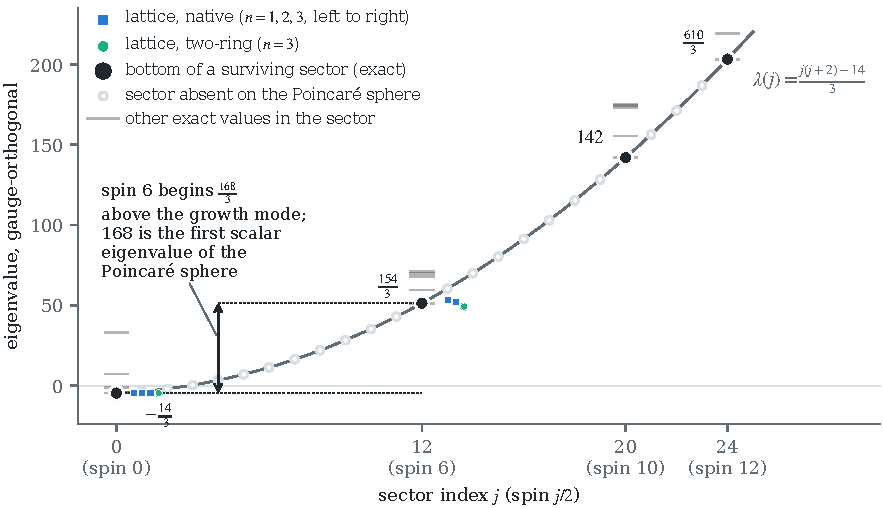
\includegraphics[width=0.95\textwidth]{figures/fig_spectrum_ladder.pdf}
  \caption{The gauge-orthogonal spectrum at the Berger field, sector by sector. Curve:
  $\lambda(j)=(j(j+2)-14)/3$. Filled: the bottom of each sector that survives on the Poincar\'e sphere;
  hollow: sectors the icosahedral group forbids; grey ticks: the other exact values of a surviving
  sector. Squares and circles: lattice eigenvalues near the \reddel{bottom of spins $0$ and $6$}\redins{left-invariant values and the lowest gauge-orthogonal values of spin $6$} from the two
  lattice forces of~\cite{davisrtc} (native $n=1,2,3$; two-ring $n=3$).}
  \label{fig:ladder}
\end{figure}

\section{The floor across the Berger family}\label{sec:family}

The computation above never used the value $3$ except through $g_0$. Replace it by any stretch $t>0$:
the Berger metric $g=(t,1,1)$, its Levi-Civita field, and the same circular top-weight field $b$.

\begin{proposition}[The floor law]\label{prop:family}
For every $t>0$ and every $j\ge0$, the field $b=f\,(\hat\theta^1+i\hat\theta^2)\otimes(\tau_1+i\tau_2)$ is an
eigenvector of $H$ at the Berger field of $(t,1,1)$, orthogonal to every gauge direction, with eigenvalue
\[
  \boxed{\;\lambda_t(j)\;=\;\frac{j(j+2)-2(t-3)\,j-2(t-2)(t+4)}{t}\;}
\]
At $t=3$ this is $\lambda(j)$ of Proposition~\ref{prop:bottom}.
\end{proposition}
\begin{proof}
The proof of Proposition~\ref{prop:bottom}, with $t$ symbolic in place of $3$. The block on the squashed
plane has eigenvalues $\lambda_t(j)$, $(j^2+4jt-8j-2t^2-4t+16)/t$ and
$(j^2+jt+5t^2-4t\pm t\sqrt{j^2+t^2})/t$\redins{ (the last three of the compression only)}. The first has eigenvector $(-1,-i,-i,1)$, and the three facts
listed there (no coupling to the $\tau_0$ component of $b_0$, no leak into the next weight, and
orthogonality to every gauge direction) hold as identities in $j$ and $t$
(\path{scripts/ricci_su2_sector_formula_squashed.py}).
\end{proof}

The Weitzenb\"ock identity of Lemma~\ref{lem:weitz} holds on every Berger sphere, and it explains the
shape of the floor law.

\begin{proposition}[The twist is a lowest Landau level]\label{prop:landau}
Let $t>0$.
\begin{enumerate}
  \item In every sector, $H+GG^*=\sum_iX_i^*X_i+R_0(t)$ with $X_i=\rho_i/\sqrt{g_i}+\Omega_i$, where $R_0(t)$ is a
    constant real symmetric $9\times9$ matrix with eigenvalues $12-8t$ $(\times2)$, $4(t-1)$,
    $-2\bigl(\sqrt{2t^2-2t+1}-1\bigr)$ $(\times2)$, $2\bigl(\sqrt{2t^2-2t+1}+1\bigr)$ $(\times2)$ and
    $3t-2\pm\sqrt{9t^2-4t+4}$. For $t\ge12/7$, $12-8t$ is the lowest of them.
  \item Write $b=f\otimes\beta$, with $\beta$ the internal frame $(\hat\theta^1+i\hat\theta^2)\otimes(\tau_1+i\tau_2)$,
    and $X_\pm=X_1\pm iX_2$. Then
    \[
      X_+b=0,\qquad X_0b=i\kappa\,b,\quad \kappa=\frac{2t-4-j}{\sqrt t},\qquad R_0(t)\beta=(12-8t)\beta .
    \]
  \item Consequently, \redins{for $\norm b=1$, }in the identity of (1), the fibre term of $b$ is $\norm{X_0b}^2=\kappa^2$, the curvature term
    is $12-8t$, and the transverse term is $\norm{X_1b}^2+\norm{X_2b}^2=2(j+t)$:
    \[
      \lambda_t(j)=\kappa^2+2(j+t)+(12-8t).
    \]
\end{enumerate}
\end{proposition}
\begin{proof}
(1) The proof of Lemma~\ref{lem:weitz} with $t$ symbolic: every coefficient of degree one and two agrees in
$U(\su)$, identically in $t$ (\path{scripts/ricci_su2_weitzenbock_symbolic_t.py}). The eigenvalues are those of
the symbolic $R_0(t)$, and the comparison is elementary. (2) $(\rho_1+i\rho_2)f=0$ because $f$ is the top weight,
and $(\Omega_1+i\Omega_2)\beta=0$, $\Omega_0\beta=i(2t-4)\beta/\sqrt t$ and $R_0(t)\beta=(12-8t)\beta$ hold as
identities in $t$; $\rho_0f=-ij f$ (\path{scripts/ricci_su2_landau_symbolic.py}). (3) follows from (1), (2) and
Proposition~\ref{prop:family}.
\end{proof}

\begin{remark}
In the language of a charged particle in a magnetic field, $X_+b=0$ is the lowest-Landau-level condition for the
two transverse covariant derivatives, $\kappa$ is the momentum along the fibre, and $12-8t$ is the most negative
curvature the internal frame can see (for $t\ge12/7$). The fibre term alone is smallest where the momentum
vanishes, at $j=2t-4$; the transverse term $2j$ moves the minimum of $\lambda_t(j)$ over $j$ to $j=t-4$
(Corollary~\ref{cor:family}). The statement that
$b$ is the \emph{floor} is not implied by (2): it needs every other state of the sector to cost more, which is
Theorem~\ref{thm:range}.
\end{remark}

The certificate of Theorem~\ref{thm:gap} takes $t$ as a parameter; run at $t=3$ it reproduces
Table~\ref{tab:cert} exactly (\path{scripts/ricci_su2_gap_certificates_t.py}). At a second squashing it gives the same kind of
complete statement.

\begin{theorem}[The Floor Theorem at $(4,1,1)$]\label{thm:t4}
At the Berger metric $g=(4,1,1)$:
\begin{enumerate}
  \item the Weitzenb\"ock identity of Lemma~\ref{lem:weitz} holds with $R_0$ of eigenvalues $-20$
    $(\times2)$, $-8$ $(\times2)$, $12$ $(\times3)$ and $10\pm2\sqrt{33}$, and $\omega^2=36$; every
    gauge-orthogonal eigenvalue in the sector of spin $j/2$ is at least $(\sqrt{j(j+2)/4}-6)^2-20$ whenever
    $\sqrt{j(j+2)/4}\ge6$;
  \item for $j=0,12,20,24,30,32$, $\lambda_4(j)=j^2/4-8$ is the lowest gauge-orthogonal eigenvalue of its
    sector, and every other eigenvalue of $H+GG^*$ is at least $\lambda_4(j)+1/3-10^{-53}$;
  \item on the Poincar\'e sphere, the gauge-orthogonal spectrum below $136$ consists of the spin-$0$ values
    $-8$ $(\times2)$, $22-2\sqrt{129}$, $29/5$ $(\times2)$ and $22+2\sqrt{129}$, the spin-$6$ values from $28$
    upward and the spin-$10$ values from $92$ upward; spin $12$ begins exactly at $136$.
\end{enumerate}
\end{theorem}
\begin{proof}
As for Theorem~\ref{thm:gap}. The six sectors certify with exactly four negative pivots each,
$\varepsilon\reddel{\le8.7\times10^{-54}}\redins{<1.3\times10^{-55}}$ and smallest pivot \reddel{$0.65$}\redins{at least $0.649$}. The tail bound exceeds $136$ from $j=36$ on:
exactly, $\sqrt{342}-6>\sqrt{156}$, with margin $0.0032$ in that form. The spin-$0$ slice is computed in exact
arithmetic (receipts in \path{research/su2-floor-family-20261119/}).
\end{proof}

So at $t=4$ \redins{the Poincar\'e sphere }\reddel{there are}\redins{has} still exactly three growth directions, and the floor gap is $36$. Unlike $t=3$, spin $6$
begins below the top of the spin-$0$ spectrum, so the sectors interleave there.

\paragraph{The floor law over a range.} A certificate need not be taken one $t$ at a time. For a slice
$t\in[a,b]$, enclose $A(t)-\lambda_t(j)-\delta$ for \emph{all} $t$ in the slice at once, with $t$ and
$\lambda_t(j)$ entered as intervals, and proceed as in the proof of Theorem~\ref{thm:gap}. Bound the
perturbation by $\rho=\min(\text{Frobenius},\text{maximal row sum})$ of the enclosure radii; both bound the
$2$-norm of a symmetric perturbation\redins{. As in Theorem~\ref{thm:gap}, the radii are taken about the stored
midpoints, and $\rho$, the residual $\norm{M-LDL^\top}_F$ and $\varepsilon$ are evaluated with outward rounding}. Then exactly four negative pivots and $\varepsilon<\delta$ give, for every
$t$ in the slice, at most two eigenvalues below $\lambda_t(j)+\delta-\varepsilon$. By
Proposition~\ref{prop:family}, both copies of $\lambda_t(j)$ are among them.

\paragraph{Charge blocks.} The rotation about the long axis, acting at once on the sector, the frame index
and the Lie index, is a symmetry of the Berger field. Its charge makes the certificate independent of the size of
the sector. Take $\rho_0,\rho_1,\rho_2=-2iJ_z,-2iJ_x,-2iJ_y$ on $V_j$ (equivalent to the representation used so
far: same brackets), with weights $m\in\{-l,\dots,l\}$, $l=j/2$, and take the frame and Lie indices in the
eigenbasis of the rotation, with charges $c_f,c_l\in\{-1,0,1\}$.

\begin{lemma}[Charge blocks]\label{lem:charge}
Let $t>0$ and $c=c_f+c_l$. In this basis $\Omega_0=i\operatorname{diag}\bigl(c(t-2)/\sqrt t\bigr)$, $\Omega_+$
raises $c$ by exactly one, $\Omega_-$ lowers it by exactly one, every nonzero entry of $\Omega_\pm$ has modulus
$\sqrt{2t}$, and $R_0(t)$ preserves $c$. Hence $H+GG^*$ preserves the charge $q=m+c$, and the sector of spin $j/2$
is the orthogonal sum of the charge blocks, each spanned by the at most nine states $(m,c_f,c_l)$ with
$m=q-c_f-c_l$, $|m|\le l$. The state of charge $l+2$ is the twist $b$ alone, and the state of charge $-l-2$ its
conjugate.
\end{lemma}
\begin{proof}
Exact, with $t$ symbolic (\path{scripts/ricci_su2_charge_selection_symbolic.py}). \redins{For every $j$, the antiunitary map $J\otimes K$, with $J$ the real ($j$ even) or quaternionic ($j$ odd)
structure of $V_j$ and $K$ complex conjugation on the frame and Lie indices, commutes with $H+GG^*$, whose
coefficients are real, and reverses the charge; so the block of charge $-l-2$ has the same entry as the twist's.
}Since $\rho_0$ is diagonal and
$\rho_1\pm i\rho_2=-2iJ_\pm$ shifts $m$ by $\pm1$, each of $X_0$ and $X_\pm$ shifts $q$ by $0$ or $\pm1$, and
$\sum_iX_i^*X_i=X_0^*X_0+\tfrac12(X_+^*X_++X_-^*X_-)$ preserves $q$; so does $R_0(t)$.
\end{proof}

\begin{remark}[Why the floor formula is exact]\label{rem:counting}
Lemma~\ref{lem:charge} explains Propositions~\ref{prop:bottom} and~\ref{prop:family}, which were proved by
symbolic computation. The twist is the only state of charge $l+2$, so it spans a $1\times1$ block and is an
eigenvector of $H+GG^*$. The gauge map preserves the charge, with the gauge parameter $\xi$ carrying the weight
and the Lie index only, so its charges reach $l+1$ at most. Hence $G^*b=0$, and $Hb=(H+GG^*)b$: the twist is an
exact gauge-orthogonal eigenvector of $H$, and its eigenvalue is its diagonal entry. The argument uses only the
rotation about the long axis, so it holds for any left-invariant background with that symmetry. Whether the twist
is the \emph{floor} is a separate statement, and it depends on the background (Section~\ref{sec:family},
``Further observations'').
\end{remark}

\begin{theorem}[The floor law on $2.75\le t\le10$]\label{thm:range}
For every $t\in[2.75,10]$ and every $j\ge0$, $\lambda_t(j)$ is the
lowest eigenvalue of $H+GG^*$ in the sector of spin $j/2$, with multiplicity exactly two, and the lowest
gauge-orthogonal eigenvalue there.
\end{theorem}
\begin{proof}
By Lemma~\ref{lem:charge} it suffices to show that every charge block other than the two twist blocks has
all its eigenvalues above $\lambda_t(j)$; the two twist blocks are $1\times1$ with entry $\lambda_t(j)$
(Proposition~\ref{prop:family}).

\emph{Sectors $j\le99$.} Each block is enclosed for all $t$ in a slice at once and certified positive
definite after the shift $\lambda_t(j)+\eta$, as described above\redins{ ($\eta>0$ plays the role of $\delta$ there, chosen per block and slice as half the double-precision gap)}, with no negative pivot and $\varepsilon<\eta$
(\path{scripts/ricci_su2_block_interval_cert.py}). For $j\le40$, $943$ blocks and $12{,}596$ block-slices, smallest
margin $\eta-\varepsilon=1.7\times10^{-5}$ (receipt \path{block_cert_j40.json}); for $41\le j\le99$, $4{,}307$
blocks and $36{,}166$ block-slices, smallest margin $2.9\times10^{-3}$ (receipt \path{block_cert_j41_99.json}).

\emph{Sectors $j\ge100$.} Write $m=l-x$. The row of $(m,c_f,c_l)$ and the row of $(-m,-c_f,-c_l)$ have the same
quantity $G$ below ($x\mapsto2l-x$, exactly), so $0\le x\le l$ suffices. For the state of type $(c_f,c_l)$, the diagonal entry of its block minus $\lambda_t(j)$ minus
the sum of the moduli of its off-diagonal entries (its Gershgorin radius) is, identically in $l$, $x$ and $t$,
\[
  G=4x(2l-x)\Bigl(1-\frac1t\Bigr)+\frac{4l(2-c)(t-2)}{t}+E-2\sqrt{2t}\Bigl[n_-\sqrt{x(2l-x+1)}+n_+\sqrt{(2l-x)(x+1)}\Bigr],
\]
with $E=c^2(t-2)^2/t+4c(t-2)x/t+C_a-R_a+2(t-2)(t+4)/t$, where $C_a$ is the diagonal entry of
$-(\Omega_1^2+\Omega_2^2)+R_0(t)$, $R_a$ the sum of the moduli of its other entries in the same row, and $n_\pm$ the
numbers of nonzero entries of $\Omega_\pm$ in the column of the type
(\path{scripts/ricci_su2_charge_selection_symbolic.py}; the nine types are tabulated in
\path{scripts/ricci_su2_floor_large_j.py}). If $G>0$ on every row except the twist, every other block lies above
$\lambda_t(j)$ by Gershgorin's theorem. For $l\ge50$ and $t\in[2.75,10]$ this is proved by bisection in interval
arithmetic: for $x\le20$ on $(1/l,t)$, $G/l>5.9\times10^{-4}$ ($373$ boxes); for $x\ge20$, after dividing by $lx$, on
the relaxed box $(x/l,1/l,1/x,t)\in[0,1]\times[0,1/50]\times[0,1/20]\times[2.75,10]$, $G/(lx)>0.85$ ($9$ boxes)
(receipt \path{floor_large_j.json}).

Receipts are in \path{research/su2-floor-family-20261119/}. Independently, a first certificate on the full
sector matrices of the fifteen sectors $j\le12$, $20$, $24$ agrees: $1{,}091$ slices tile $[2.75,10]$ exactly in each of the fifteen sectors, the finest $0.002$ wide near
$t=2.75$, where the gap above the floor is smallest ($0.16$ for $j=4$, $0.18$ for $j=1$). Every slice has
exactly four negative pivots and $\varepsilon<\delta$, the smallest margin $\delta-\varepsilon$ being $0.0018$.
A degenerate slice at $t=3$ reproduces Table~\ref{tab:cert}
(\path{scripts/ricci_su2_floor_interval_cert.py}, receipt
\path{research/su2-floor-family-20261119/interval_cert_2.75_10.json}).
\end{proof}

At $t=3$ this completes Proposition~\ref{prop:bottom}: $(j(j+2)-14)/3$ is the floor of every sector of the
Berger field $(3,1,1)$, not only of those that survive on the Poincar\'e sphere.

\begin{remark}[Below the range]\label{rem:tstar}
There are two thresholds, one for each statement of Theorem~\ref{thm:range}.
\emph{Gauge-orthogonal spectrum.} In double precision, $\lambda_t(j)$ is its bottom in every sector $j\le40$ for
every $t\in[2.7,2.75]$ tested. Below $t^*\approx2.6980$ (located by bisection) a lower eigenvalue appears, first
in the sector $j=4$; at $t\le2$ the branch is the floor of no sector.
\emph{The operator $H+GG^*$.} The threshold is algebraic. The charge-$0$ block of the sector $j=4$ has
$\lambda_t(4)$ as an eigenvalue exactly when $s=\sqrt t$ is a root of its determinant, whose largest positive root
is that of
\[
  3s^{16}+121s^{14}+1066s^{12}-2836s^{10}-18624s^8+20992s^6+181248s^4-425984s^2+262144,
\]
$t_A=s^2=2.7311222782\ldots$ (\path{scripts/ricci_su2_tstar_exact.py}). In double precision, below $t_A$ that
block has an eigenvalue under $\lambda_t(4)$, and between $t_A$ and $2.75$ no sector $j\le40$ has one
(\path{scripts/ricci_su2_tA_scan.py}). So between $t^*$ and $t_A$ the eigenvalue of $H+GG^*$ below
$\lambda_t(4)$ is not gauge-orthogonal, and the twist remains the floor of the slice. Only the range of
Theorem~\ref{thm:range} is certified.
\end{remark}

\begin{corollary}\label{cor:family}
Where $\lambda_t(j)$ is the floor:
\begin{enumerate}
  \item \emph{The floor gap.} On the Poincar\'e sphere, $\lambda_t(12)-\lambda_t(0)=(240-24t)/t$: $168/3$ at
    $t=3$, $36$ at $t=4$, and $0$ at $t=10$. The relation to the first scalar eigenvalue holds at $t=3$
    only, and characterises it (Remark~\ref{rem:casimir}).
  \item \emph{Where a twist goes free.} $\lambda_t(j)=0$ exactly at
    \[
      t_j=\tfrac12\Bigl(\sqrt{(j+2)^2+2(j+4)^2}-(j+2)\Bigr),
    \]
    and $\lambda_t(j)<0$ for $t>t_j$. The values are $t_3=3.045$,
    $t_4=3.403$, inside the range of Theorem~\ref{thm:range}. The same formula gives $t_0=2$,
    $t_1=2.341$ and $t_2=2.690$. These are zeros of the branch $\lambda_t(j)$ outside the certified range: at
    $t_0$ the branch is not the floor (Remark~\ref{rem:tstar}), the double-precision scan already finds a lower
    eigenvalue in the sector $j=1$ at $t=2.5>t_1$, and at $t_2$ that the branch is the floor is numerical only. At stretch
    $t$, every sector with $j<(t-4)+\sqrt{3t^2-4t}$ has negative floor. Each floor crosses zero linearly in
    $t-t_j$.
  \item \emph{The softest sector moves.} Over $j$, $\lambda_t(j)$ is smallest near $j=t-4$.
\end{enumerate}
\end{corollary}
\begin{proof}
Algebra on the formula of Proposition~\ref{prop:family}; the statements about floors hold where
Theorem~\ref{thm:range} or Theorem~\ref{thm:t4} applies.
\end{proof}

\begin{remark}[The Casimir point]\label{rem:casimir}
The cost of lifting the twist from the left-invariant sector to the sector of spin $j/2$ splits as
\[
  \lambda_t(j)-\lambda_t(0)=\Bigl(\frac{j^2}{t}+2j\Bigr)-\frac{4(t-2)}{t}\,j .
\]
The first term is the eigenvalue of the scalar Laplacian of $(t,1,1)$ on the top-weight vector $f$
(since $-\rho_0^2f=j^2f$ and $-\sum_i\rho_i^2=j(j+2)$); the second couples the weight along the long axis to the
stretch. The lift equals the round Casimir divided by the stretch, $j(j+2)/t$, for every $j$ if and only if
$t=3$. So at $t=3$ the floor gap on the Poincar\'e sphere is $\lambda_1(\Delta_{S^3/2I})/3$ because there the
lift depends on $j$ only through the Casimir. At $t=2$ the coupling vanishes: the lift is exactly the scalar
Laplacian on $f$, and $\lambda_2(0)=0$.
\end{remark}

\begin{figure}[t]
  \centering
  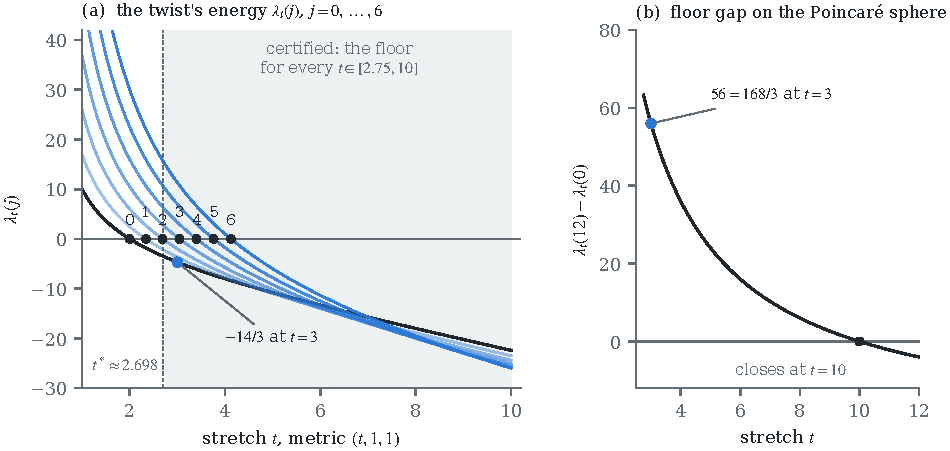
\includegraphics[width=\textwidth]{figures/fig_floor_family.pdf}
  \caption{The floor law across the Berger family. (a) $\lambda_t(j)$ for $j=0,\dots,6$; dots mark where each
  twist goes free ($t_j$); shaded: the range of Theorem~\ref{thm:range}; dashed: $t^*$ of
  Remark~\ref{rem:tstar}. (b) The floor gap on the Poincar\'e sphere, $(240-24t)/t$.}
  \label{fig:family}
\end{figure}

\paragraph{Further observations (double precision; not certified).} Two numerical experiments locate what
the floor law is and is not (scripts and receipts in the repository; see the availability section).
\begin{itemize}
  \item \emph{Landscape, not dynamics.} Under the gauge-fixed linearised flow with the operator held at the
    Berger field, a disturbance in sector $j$ decays for $t<t_j$, grows for $t>t_j$, and turns into the twist
    (overlap $1.000$ in every run). Under the actual Yang--Mills flow the Berger field is not at rest. It
    collapses towards a flat field within flow time $0.1$ (energy $34.6\to0.73$ at $t=3.55$), faster than any
    twist grows, and the disturbance decays. The floor law describes the second variation at the Berger
    field. It is not by itself a dynamical transition.
  \item \emph{Resting fields.} Among left-invariant fields on $(t_1,t_2,1)$, a multistart search
    ($36$ shapes, axis ratios up to $20$) finds \reddel{exactly three Yang--Mills fields up to gauge: two flat, and one
    non-flat relative of the meron. That relative keeps Morse index $1$ throughout, including along
    $(t,1,1)$ for $t\in[0.05,10]$, and no sector $j\le12$ crosses zero on it.}\redins{three clusters of Yang--Mills
    fields up to constant gauge rotation: the flat field $A=0$; the flat pure-gauge field $A=g^{-1}dg$, which is
    gauge-equivalent to $0$ under a non-constant gauge transformation but not under a constant one; and one non-flat
    relative of the meron. A multistart search is evidence, not a classification. In every sector and at every
    stretch checked, the relative has exactly one negative eigenvalue of $H+GG^*$, in the left-invariant sector: for
    $j\le12$ at $t=0.05,0.10,\dots,10$ along $(t,1,1)$, and for $j\le8$ on the $36$ uneven shapes. No eigenvalue of
    the sectors $1\le j\le12$ is negative at these points; crossings between the sampled stretches are not
    excluded.}
  \item \emph{Symmetry does not make the floor.} The squashed meron has the same rotation symmetry, so by
    Remark~\ref{rem:counting} the twist is an exact gauge-orthogonal eigenvector there too. Yet on the grid
    $t=0.05,0.10,\dots,10$ it is the floor of no sector $j\le12$ at any point. For $t\le1$ it is the top of every
    sector $j\le12$, and it descends as $t$ grows without reaching the bottom. On the Berger field the same scan finds it
    the floor of every sector $j\le12$ at exactly the grid points $t\ge2.70$. The difference lies in the curvature term. In
    the Weitzenb\"ock form~\cite{bl1981}, $R_0=\mathrm{Ric}-2[F,\cdot\,]$, with
    $([F,\cdot\,]b)_i=\sum_j[F_{ij},b_j]$: the Ricci curvature plus the field
    strength with the factor $2$ of the Hessian (checked to $4\times10^{-15}$ on both fields). On the twist's internal
    frame the Ricci share is $4-2t$ on both fields. The field-strength share is $8-6t$ on the Berger field (total
    $12-8t$), but positive on the squashed meron, between $0.4$ and $1.3$ for $t$ from $2$ to $8$
    (\path{scripts/ricci_su2_test2_family.py}, \path{scripts/ricci_su2_gyromagnetic_split.py},
    \path{scripts/ricci_su2_meron_ceiling_check.py}).
\end{itemize}

\section{Checks}\label{sec:checks}

\paragraph{The round sphere.} At $g=(1,1,1)$ the Levi-Civita connection is a Yang--Mills field (the
meron), and the same construction gives $-2$, $1$, $6$, $7$ and $10$ \redins{as the lowest gauge-orthogonal eigenvalues of the sectors $j=0,\dots,4$, }in spins $0$ to $2$. That is the
published fluctuation spectrum~\cite{klc2021}. It has exactly one negative eigenvalue, so index one,
as Laquer's theorem requires for a group manifold~\cite{laquer1984}. Without the commutator it gives
the coexact $1$-form spectrum of the unit $S^3$: $j^2$ and $(j+2)^2$ with their multiplicities, and
gauge zeros.

\paragraph{Lattice computations.} The two lattice Yang--Mills forces of~\cite{davisrtc}, linearised
at the Berger field on triangulations of the Poincar\'e sphere, resolve the left-invariant sector and
\reddel{the bottom of spin $6$}\redins{two eigenvalues of $H$ in spin $6$: $154/3=51.33$, the floor, and $59.52$, beside the second gauge-orthogonal value $59.50$; $H$ itself has lower, gauge-dominated eigenvalues there, and these two are matched by value} (Table~\ref{tab:lattice}). At $n=1,2$ every left-invariant mode was identified
by its eigenvector, as the lattice eigenvector with the largest overlap with the nine discrete
left-invariant directions (overlap $0.76$ to $0.999$). The mode $16-2\sqrt{73}$ is split by the
non-symmetric lattice Jacobian, between a real eigenvalue and a complex pair. The lattice linearises
the force in link coordinates at a field that is not at rest, where its Jacobian differs from the
Hessian by a term proportional to the gradient; so it is compared with the full Hessian $H$, not with
the slice.

\begin{table}[t]\centering\small
\caption{Exact eigenvalues of $H$ at the Berger field against the real part of the lattice
eigenvalue~\cite{davisrtc}. $^{\mathrm g}$: pure gauge; $^{\mathrm m}$: a mixture. At $n=1,2$ the
spin-$0$ entries are identified by eigenvector; at $n=3$, and for spin $6$, by value.}
\label{tab:lattice}
\begin{tabular}{lcrrrr}\toprule
Exact & mult. & native $n=1$ & native $n=2$ & native $n=3$ & two-ring $n=3$ \\ \midrule
\multicolumn{6}{l}{\emph{spin $0$}}\\
$-14/3=-4.6667$ & 2 & $-4.475$ & $-4.651$ & $-4.661$ & $-4.651$ \\
$(29-\sqrt{1345})/3=-2.5581^{\mathrm m}$ & 2 & $-2.191$ & $-2.504$ & $-2.529$ & $-2.529$ \\
$16-2\sqrt{73}=-1.0880$ & 1 & $-0.674\pm0.80i$ & $-1.041$ & $-1.088$ & $-1.084$ \\
$8^{\mathrm g}$ & 1 & $7.083$ & $7.869$ & $7.954$ & $7.931$ \\
$(29+\sqrt{1345})/3=21.891^{\mathrm m}$ & 2 & $20.71$ & $21.77$ & $21.86$ & $21.80$ \\
$16+2\sqrt{73}=33.088$ & 1 & $32.64$ & $33.44$ & $33.29$ & $33.16$ \\ \midrule
\multicolumn{6}{l}{\emph{spin $6$, full Hessian}}\\
$51.33$ & 2 & --- & $53.41$ & $52.27$ & $49.27$ \\
$59.52$ & 2 & --- & $61.92$ & $60.69$ & $57.50$ \\
\bottomrule\end{tabular}
\end{table}

\section{Discussion}\label{sec:discussion}

\paragraph{Scope.} The result concerns the classical linearised operator. At a field that is not at
rest, how gauge directions are separated from physical ones is a choice; the theorem is stated for the
$L^2$ (Coulomb) slice, and the full Hessian is given alongside. The theorem is not a statement about the
quantum theory and not a Yang--Mills mass gap.

\paragraph{What is special.} The value $(j(j+2)-14)/3$ is tied to $t=3$, but the mechanism is not. The
circular eigenvector uses only the rotation symmetry about the long axis and the top weight, so it is an
exact eigenvector at every squashing (Proposition~\ref{prop:family}), with the stretch entering the formula
rationally, and it is a lowest Landau level at every squashing (Proposition~\ref{prop:landau}). Whether
it is the \emph{floor} depends on $t$, and on the background: symmetry alone does not make it the floor
(Section~\ref{sec:family}, ``Further observations''). It is the floor throughout $[2.75,10]$ in every sector, and (numerically) not the floor of every sector below
$t^*\approx2.698$, where the sector $j=4$ is the first to have a lower eigenvalue. At the round metric
and at $(2,1,1)$ other modes are lower. The relation to the Poincar\'e sphere's first scalar eigenvalue, $168/3$,
is special to $t=3$, the unique stretch at which the lift of the twist depends only on the Casimir
(Remark~\ref{rem:casimir}); in general the floor gap is $(240-24t)/t$.

\paragraph{The landscape and the flow.} The Berger field is not at rest, and under the Yang--Mills flow it
slides towards a flat field faster than any twist grows (Section~\ref{sec:family}). So the floor law is a
statement about the second variation at the Berger field, the shape of the landscape there. Its non-flat
resting relative, the squashed meron, \reddel{keeps a single unstable direction across the family, and no twist goes
soft on it}\redins{has a single unstable direction in every sector and at every stretch sampled ($j\le12$), and no
twist goes soft on it there}.

\paragraph{Open questions.} The floor outside $[2.75,10]$; the gauge-orthogonal threshold $t^*$ in closed form (that of
$H+GG^*$ is algebraic, Remark~\ref{rem:tstar}); the floor along the Ricci flow of the metric; Yang--Mills fields that
are not left-invariant on the squashed spheres, where a twist might go soft at rest; and the higher eigenvalues
of each sector.

\section*{Funding and competing interests}
This work received no funding. The author declares no competing interests.

\section*{Code and data availability}
All programs and certificates are in the \textsc{GIGI} repository,
\url{https://github.com/nurdymuny/gigi}\redins{ (tag \texttt{floor-theorem-v2}; the scripts are on that tag, not yet on the main branch)}, with their outputs in
\path{research/su2-left-invariant-sector-20261119/}:
\begin{itemize}
  \item the left-invariant sector: \path{scripts/ricci_su2_left_invariant_sector.py};
  \item the sector matrices: \path{scripts/ricci_su2_spin_sector.py};
  \item gauge content: \path{scripts/ricci_su2_sector_gauge_check.py};
  \item Proposition~\ref{prop:bottom}: \path{scripts/ricci_su2_sector_formula.py};
  \item the spin-$0$ slice and the double-precision range: \path{scripts/ricci_su2_sector_minimality.py};
  \item Lemma~\ref{lem:weitz} and the certificates: \path{scripts/ricci_su2_gap_certificates.py}.
\end{itemize}
For Section~\ref{sec:family}, with outputs in \path{research/su2-floor-family-20261119/}:
\begin{itemize}
  \item Proposition~\ref{prop:family}: \path{scripts/ricci_su2_sector_formula_squashed.py};
  \item Theorem~\ref{thm:t4}: \path{scripts/ricci_su2_gap_certificates_t.py} (any rational $t$);
  \item Theorem~\ref{thm:range}: \path{scripts/ricci_su2_floor_interval_cert.py} (fifteen sectors),\\
    \path{scripts/ricci_su2_block_interval_cert.py} ($j\le99$),\\
    \path{scripts/ricci_su2_floor_large_j.py} ($j\ge100$);
  \item Proposition~\ref{prop:landau}: \path{scripts/ricci_su2_weitzenbock_symbolic_t.py},\\
    \path{scripts/ricci_su2_landau_symbolic.py};
  \item Lemma~\ref{lem:charge}: \path{scripts/ricci_su2_charge_selection_symbolic.py};
  \item the charge blocks: \path{scripts/ricci_su2_charge_block_direct.py};\\
    their closed-form rows: \path{scripts/ricci_su2_block_rows_symbolic.py};
  \item Remark~\ref{rem:tstar}: \path{scripts/ricci_su2_floor_family_scan.py},
    \path{scripts/ricci_su2_tstar_exact.py}, \path{scripts/ricci_su2_tA_scan.py};
  \item the flow experiment: \path{scripts/ricci_su2_soft_mode_flow.py};
  \redins{\item the outward error budget of every certificate: \path{scripts/ricci_su2_outward.py}, with its
    adversarial tests in \path{scripts/ricci_su2_outward_test.py};}
  \redins{\item the resting relative's index for $t<1$: \path{scripts/ricci_su2_meron_index_below1.py};}
  \item symmetry does not make the floor:\\ \path{scripts/ricci_su2_test2_family.py},
    \path{scripts/ricci_su2_gyromagnetic_split.py},\\ \path{scripts/ricci_su2_meron_ceiling_check.py};
  \item resting fields: \path{scripts/ricci_su2_resting_fields.py},
    \path{scripts/ricci_su2_resting_fields_general.py}, \path{scripts/ricci_su2_meron_family_soft.py}.
\end{itemize}
This paper, its source, and the code and data above are archived on Zenodo under the concept DOI
\url{https://doi.org/10.5281/zenodo.24386613}, which resolves to the latest version.

\begin{thebibliography}{99}\small
\bibitem{bar1992} C.~B\"ar, The Dirac operator on homogeneous spaces and its spectrum on $3$-dimensional lens spaces, \emph{Arch.\ Math.} 59 (1992) 65--79.
\bibitem{bl1981} J.-P.~Bourguignon, H.~B.~Lawson, Stability and isolation phenomena for Yang--Mills fields, \emph{Comm.\ Math.\ Phys.} 79 (1981) 189--230.
\bibitem{davisrtc} B.~R.~Davis, Reading the curve, not counting the points: a two-ring Petrov--Galerkin curvature force for discrete Yang--Mills dynamics on the Poincar\'e homology sphere, 2026, \url{https://doi.org/10.5281/zenodo.24328085}.
\bibitem{henkellauret2026} J.~Henkel, E.~A.~Lauret, Hodge Laplacian on $1$-forms of homogeneous $3$-spheres, 2026, \href{https://arxiv.org/abs/2605.05406}{arXiv:2605.05406}.
\bibitem{hitchin1974} N.~Hitchin, Harmonic spinors, \emph{Adv.\ Math.} 14 (1974) 1--55.
\bibitem{klein1884} F.~Klein, \emph{Vorlesungen \"uber das Ikosaeder und die Aufl\"osung der Gleichungen vom f\"unften Grade}, Teubner, Leipzig, 1884.
\bibitem{klingschueth2022} J.~Kling, D.~Schueth, On the Dirac spectrum of homogeneous $3$-spheres, \redins{\emph{J.\ Geom.\ Anal.} (2022), \href{https://doi.org/10.1007/s12220-022-00997-x}{doi:10.1007/s12220-022-00997-x}, }\href{https://arxiv.org/abs/2204.12990}{arXiv:2204.12990}.
\bibitem{klc2021} \reddel{S.~Kumar}\redins{K.~Kumar}, O.~Lechtenfeld, G.~Pican\c{c}o Costa, Instability of cosmic Yang--Mills fields, \emph{Nucl.\ Phys.\ B} 973 (2021) 115583, \href{https://arxiv.org/abs/2102.08401}{arXiv:2102.08401}.
\bibitem{lachiezerey2004} M.~Lachi\`eze-Rey, Eigenmodes of dodecahedral space, \reddel{2004}\redins{\emph{Class.\ Quantum Grav.} 21 (2004) 2455--2464}, \href{https://arxiv.org/abs/gr-qc/0402035}{arXiv:gr-qc/0402035}.
\bibitem{laquer1984} H.~T.~Laquer, Stability properties of the Yang--Mills functional near the canonical connection, \emph{Michigan Math.\ J.} 31 (1984) 139--159.
\bibitem{lauret2019} E.~A.~Lauret, The smallest Laplace eigenvalue of homogeneous $3$-spheres, \redins{\emph{Bull.\ Lond.\ Math.\ Soc.} 51 (2019) 49--69, }\href{https://arxiv.org/abs/1801.04259}{arXiv:1801.04259}.
\bibitem{mpmath} The mpmath development team, mpmath: a Python library for arbitrary-precision floating-point arithmetic, \url{https://mpmath.org}.
\bibitem{ohnitapan1989} Y.~Ohnita, Y.~L.~Pan, On weakly stable Yang--Mills fields over positively pinched manifolds and certain symmetric spaces, \reddel{preprint MPI/89-49, Max-Planck-Institut f\"ur Mathematik, Bonn, 1989}\redins{\emph{Kodai Math.\ J.} 13 (1990) 317--332}.
\end{thebibliography}

\end{document}
